%\documentclass[conference,final]{IEEEtran}
%\documentclass[a4paper]{article}

\documentclass{rspublic}

\usepackage[utf8]{inputenc}
%\usepackage{graphicx}                                                                                             
\usepackage{url}
\usepackage{float}
\usepackage{times}
\usepackage{multirow}
\usepackage{listings}
\usepackage{times}
\usepackage{paralist}
\usepackage{wrapfig}
\usepackage[small,it]{caption}
\usepackage{multirow}
\usepackage{ifpdf}
\usepackage{subfig}
\usepackage[pdftex]{graphicx}
\usepackage{natbib}
\usepackage{listings}
\usepackage{keyval}
\usepackage{color}


\long\def\comment#1{{ \bf \textcolor{magenta}{\bf #1}}}
\long\def\ccomment#1{{ \bf \textcolor{blue}{\bf #1 (SJ)}}}
\newcommand{\F}[1]{\B{\textcolor{red}{FIXME: #1}}}
\newcommand{\C}{\comment}
\newcommand{\CC}{\ccomment}
\newcommand{\fix}[1]{\textcolor{red}{\bf #1}}
\newcommand{\tc}{$T_c$ }
\newcommand{\tcnsp}{$T_c$}

\setlength\parskip{-0.15em}
\setlength\parsep{-0.0em}
\newcommand{\upup}{\vspace*{-0.6em}}
\newcommand{\upp}{\vspace*{-0.6em}}
\newcommand{\up}{\vspace*{-0.3em}}

\newif\ifdraft
\drafttrue

\ifdraft
\newcommand{\fixme}[1]{ { \bf{ ***FIXME: #1 }} }
\newcommand{\jhanote}[1]{ {\textcolor{red} { ***Jha: #1 }}}
\newcommand{\yyenote}[1]{ {\textcolor{blue} { ***yye00: #1 }}}
\else
\newcommand{\jhanote}[1]{}
\newcommand{\yyenote}[1]{}
\newcommand{\fixme}[1]{}
\fi

\newcommand{\jitter}[1]{{$\sigma(\alpha)$}}

\newif\ifpdf
\ifx\pdfoutput\undefined
  \pdffalse
\else
  \ifnum\pdfoutput=1
    \pdftrue
  \else
    \pdffalse
  \fi
\fi

\ifpdf
\DeclareGraphicsExtensions{.pdf, .jpg}
\else
\DeclareGraphicsExtensions{.eps}
\fi

\title{Modelling Data-driven CO$_{2}$ Sequestration Using Distributed HPC Cyberinfrastructure}

\author[el-khamra, jha]{Yaakoub el-Khamra$^{1}$,Shantenu Jha$^{2,3,4*}$ \\
  \small{\emph{$^{1}$TACC, Austin, USA} \\ \emph{$^{2}$Center for
      Computation \& Technology, Louisiana
      State University, USA}\\
    \emph{$^{3}$Department of Computer Science, Louisiana State University, USA}\\
    \emph{$^{4}$e-Science Institute, Edinburgh, UK}} \\
{\footnotesize {\hspace{0.0 in} $^*$Corresponding Author sjha@cct.lsu.edu}}}

\begin{document}

\maketitle

\begin{abstract}{ensemble simulations, sequestration, distributed
    applications, scale-out} In this paper, we layout the
  computational challenges involved in effectively simulating complex
  phenomenon such as sequestrating CO$_2$ in existing oil
  reservoirs. The challenges arise at multiple levels: (i) the
  computational complexity of simulating the fundamental processes;
  (ii) the resource requirements of the computationally demanding
  simulations; (iii) the need for integrating real-time data
  (intensive) and computational intensive simulations; (iv) and the
  need to implement all of these in a robust, scalable and extensible
  approach. We will outline the architecture and implementation of the
  solution we develop in response to these requirements, and discuss
  results to validate claims that our solution scales to effectively
  solve desired problems sizes and thus provides the capability to
  generate novel scientific insight.\end{abstract}

\section{Introduction and Motivation}

Global energy needs today present serious challenges: the increasing
demand for energy must be met, however at the same time the emissions
of greenhouse gases into the atmosphere must be reduced. Even as
alternative energy sources continue to develop and gain popularity,
the fact remains that fossil carbon resources will continue to be in
heavy use (in both developing and industrialized countries) and
consequently generate large volumes of carbon dioxide
~\citep{GeoRPT}. The atmospheric impact of this greenhouse gas can be
abated through capturing and sequestering significant fractions of the
produced CO$_2$.

For long-term storage of large volumes of CO$_2$, porous subsurface
geologic formations are ideal candidates: these are the same
formations responsible for the existence of oil and gas
reservoirs. Indeed much the technology behind carbon dioxide
sequestration (including drilling, gas injection, reservoir management
and of course reservoir simulation) stems from drilling, petroleum and
reservoir engineering. Injecting CO$_2$ into an oil-gas reservoir can
also lead to improved oil recovery by ``pushing out'' the oil and gas
for production, this allows for reduced net cost through increased
revenues from oil and gas production ~\citep{EORBook}.

One of the major areas of research in this field is the
characterization of reservoirs that are safe and secure,
environmentally and geologically and are therefore promising
candidates for CO$_2$ sequestration ~\citep{GeoRPT,Luigi}. Our efforts
are directed towards developing cyberinfrastructure tools,
technologies and abstractions that facilitate large scale reservoir
characterization and forecasting studies.  Since the amount of
information obtained directly from reservoirs is very small compared
to the actual size of the reservoir, history matching techniques have
been developed to match actual reservoir production with simulated
reservoir production, therefore obtaining a more ``satisfactory'' set
of models. One of the promising approaches to history matching is the
use of Ensemble Kalman filters (EnKF) ~\citep{KalmanPaper, DO2007,
  LiEnKF07, DO2006}. 

This paper is structured as follows: in the next we describe the basic
physical processes and parameters that are used to understand
sequestration. In the latter part of Section 2, we outline the
computational approach adopted, computational complexity and the
simulation parameter choice considerations that need to be determined.
In Section 3 we present the architecture and the specific solution we
implement to address the physical and engineering problem of CO$_2$
sequestration. The focus in this section is not on the specific
details of each component -- as each component of the solution was
developed for a different original problem(s), but on how we bring the
various components togethe.  The final section outlines some
preliminary results that validate our solution -- both computational
and scientific (inject rates for CO$_2$).

% \jhanote{Yaakoub: This is where the back-of-the-envelope quantitative
%   estimates of computational requirements will be placed. Having
%   established the scientific (and moral) imperative), we will now
%   establish the computational challenge of the problem/solution at
%   hand.}

% \begin{figure}
% \begin{center}
% \includegraphics*[scale=0.33,angle=0]{figures/3StageKalmanFilter}
% \end{center}
% \caption{Schematic illustrating the variability between stages of a typical
%   ensemble Kalman filter based simulation. The end-to-end
%   application consists of several stages; in general at each stage the
%   number of models generated varies in size and duration.}
% \label{fig:irregular_execution}
% \end{figure}

\section{Modelling CO$_2$ Sequestration}

%\subsection{Scientific Problem}

% \jhanote{The Sceintific Problem: This needs a couple of paragraphs ---
%   all about injection etc, what are the parameters etc. so that when
%   the figures are shown later, we'll know how to analyze them. This
%   should contain sufficient backgroud material that was used for the
%   e-Science 2009 talk}
% \yyenote{See computational approach paragraphs 2 and 3}

\subsection{The Computational Approach}

As mentioned earlier, CO$_2$ sequestration in oil/gas reservoirs
typically involves history matching studies to obtain a better
understanding of the reservoir geology and fluid flow properties.
At the core of the history matching process is the EnKF -- 
which are recursive filters that can be used to
handle large, noisy data; the data in this case would be the results
and parameters from ensembles of reservoir models that are sent
through the filter to obtain the ``true '' state of the data.
The data is the porosity map and the permeability tensor maps.

Since the reservoir model varies from one ensemble to another, the
run-time characteristics of the ensemble simulation are irregular and
hard to predict. Furthermore, at simulation times when real historical
data is available, all the data from the different ensembles at that
simulation time must be compared to the actual production data, before
the simulations are allowed to proceed. This translates into a global
synchronization point for all ensembles; hence performing large scale
studies for complex reservoirs in a reasonable amount of time would
benefit greatly from the use of distributed, high performance, high
throughput and on-demand computing resources.

These history matching/reservoir characterization studies are then
followed by forecast studies where CO$_2$ is injected at specified
rates and pressures based on operational and regulatory constraints.
These simulations answer key questions about the sequestration
process: where will the CO$_2$ gas flow, how much CO$_2$ can be
injected safely, what is the long term fate of the injected CO$_2$.

For our purposes we make the same simplifying assumptions about the
injected CO$_2$, as in Ref~\cite{Pawar}. Carbon dioxide is treated as
a gas phase that is soluble in oil but not water, and compositional
effects of CO$_2$ injection are ignored. In our test/demonstration
simulations, carbon dioxide is injected as a supercritical gas at 2800
psi. Regulatory constraints limit the bottom-hole injection pressure;
the bottom hole pressure at the injection point does not exceed the
hydrostatic pressure gradient by more than 0.2 psi/ft.

\subsection{Analyzing The Computational Complexity}

%\subsection{Single Machine Versus Distributed Infrastructure}

%\subsection{EnKF Scalability}

An important parameter in the EnKF workflow is the size of the
ensemble (number of ensemble members). The ensemble size should be
large enough to propagate the information contained in the
observations to the model variables. Smaller ensembles cause the
analysis error to become larger. Too small an ensemble size can give
poor approximations to the infinite ensemble case: the ensemble
covariance underestimates the error covariance substantially. This
effect can be monitored by comparing the actual forecasted model data
differences to those expected on the basis of the forecasted ensemble
covariance ~\cite{Burger98}.

In contrast, Ref~\cite{Hout98} found that while the analysis error
decreased as the number of ensembles increased, representative
ensembles can be maintained with a relatively small ensemble size
(order of hundreds) using a pair of ensembles. Furthermore, the
required ensemble size remains constant irrespective of the state
vetor size and observation size ~\cite{Mitchell02}. However, if a
small ensemble size requiring severe localization (as is sometimes the
case with reservoir models), this can cause a significant amount of
spatial incoherence.


For these reasons, optimal ensemble size is considerably difficult to
determine without any preliminary analysis. Large ensemble sizes
directly translate to increased computational cost and delays in the
time to completion. Conversely, smaller ensemble sizes, while more
efficient require prior knowledge of localization requirement for
reduced analysis errors.

\subsubsection{Analyzing the Trade-offs}  

Typically, reservoir characterization studies followed by forecast
studies are run for a reservoir management recommendation to be
made. The studies must be therefore completed within a fixed timeframe
(few weeks at best). This imposes restrictions on the size of the
ensemble used. Fortunatly, the ensemble members are independent
therefore can be run across a distributed environment. It is for this
reason that we develop a scalable autonomic framework for EnKF
applications (to be described in Section 3). The larger ensemble sizes
also increase the computational cost of the EnKF application. For that
reason, we developed a parallel EnKF.

Since the choice of ensemble size has a direct impact on total time to
completion, a tradeoff can be established: large ensembles of
small/less detailed simulations as opposed to small ensembles of
large/detailed simulations. If the ensemble is too small, it fails to
span the space of possible models and moreover the inversion tends to
be unstable. On the other hand, too-large ensembles are
inefficient. The tradeoff can keep the number of SU's required
constant, and with prior knowledge of available resources, the total
time to completion as well. 



The question becomes: given a small
time-frame of ten days for example, what ensemble size and what
problem size can be completed so that by the tenth day results can be
collected and a decision made. While we have not addressed this
problem in the workflow manager or the reservoir simulator, we have
built those tools with these tradeoffs in mind.

\subsubsection{Computational Requirement: Current Capability}

Consider a practical reservoir study that involves characterization,
production forecast and sequestration forecast. For a one million grid
cell model with our reservoir simulator, one iteration on 16 cores
requires roughly 30 seconds. Also assume we will be performing data
assimilation with observational data collected every 300 iterations.
Therefore each model takes 9000 seconds on 16 cores. With 100 ensemble
members, this equates to 900,000 seconds using 16 cores running one
ensemble at a time, or 9000 seconds on a job of 1600 cores with all
ensembles running concurrently (the details of which will be presented
later)

Assume for now that we are working with the ranger supercomputing
system at TACC. We would have access to 1600 cores for a maximum of 2
days, which should allow us to run roughly 1.6 years worth of
simulations. With 15 years of history matching, 15 years of forecasts
and another 15 years of sequestration simulation, or 29 simulations
with 1600 core size and 2 day duration. The wait time in the queue for
such a job is, on average, 30 hours (1.25 days) on ranger. If we
submit the subsequent job to the queuing system after the current job
is finished, the total duration of the entire study will therefore be
roughly 95 days (29 * (2 + 1.25)).

Certain improvements are possible obviously. Using three machines as a
distributed infrastructure instead of just one machine, based on
\ref{fig:SingleVsDistributed}, we can expect a reduction of the total
time to completion by about a third, roughly 65 days. Clearly this is
a very long time to solution and futher optimizations are both
required and possible.

\subsubsection{Computational Requirement: Typical Problems that Need to be Solved}
It is generally understood that the ensemble determines the accuracy
of the EnKF and as the ensemble size increases, the EnKF should
converge to the exact Kalman filter ~\cite{JiaLi}. This being the
case, whenever computational power and timeline restrictions permit,
larger ensembles should be used.

Consider a similar case to the one outlined earlier where instead of
one hundred ensemble members, we use one thousand. This translates to
950 days running on 1600 cores or 95 days running on 16000 cores.
This is a considerable commitment in both time and compute power. Even
in terms of energy consumption; on a bluegene L, a low power
consumption supercomputer, the total amount of energy consumed is 0.62
Giga-Watt-hours.

\section{Meeting the Requirements: Design and Architecture}

Due to the complexity of the problem, involving reservoir simulation,
geostatistics on one end, and simulation management, workflows, grid
and high-throughput computing on another, a design decision was made
early in development to make full use of existing tools and
abstractions whenever possible. This resulted in a rapid development
cycle and faster turn-over. The components we developed and use are as
follows:

\subsection{The Reservoir Simulator} 

Based on the Cactus Code~\citep{cactus_web} high performance
scientific computing framework and the Portable Extensible Toolkit for
Scientific Computing: PETSc~\citep{PETSc}, the BlackOil reservoir
simulator solves the equations for multiphase fluid flow through
porous media, allowing us to simulate the movement of oil and gas in
subsurface formations. With a few parameter changes, BlackOil is also
used for modelling the flow of CO$_2$, however it cannot simulate any
geochemical interaction. While adequate as a first order
approximation, it is still under heavy development to enable it to
satisfactorily model geochemical phenomena.

\subsection{The Ensemble Kalman filter} 

The Kalman filter and its variants are being widely adopted to address
the need for flexible, efficient inversion of nonlinear, stochastic
problems \cite{DataAssim}. However, many challenges remain,
including a better understanding of filter behavior, methods to
stabilize filters, and guidelines for optimal filter structure. In
addition, because ensembles of large, nonlinear models impose a heavy
computing burden, engineers and scientists need access to
supercomputing resources. Efficient use of these resources requires a
balanced cyber-infrastructure for ensemble inversion; the inversion
infrastructure must (1) be sensor--aware, so that inversion proceeds
when new data are available; (2) be able to manage parallel and
distributed workflow elements; (3) distribute and load--balance
simulations with a wide range of execution times; (4) move large data
sets to initialize models, compute gains, and update models; and (5)
recover from errors in ensemble member simulations.

The EnKF we use is based on Cactus and PETSc --it computes the Kalman
gain matrix and updates the model parameters of the ensembles. The
Kalman filter requires live production data from the reservoir for it
to update the reservoir models in real-time, and launch the subsequent
long-term forecast, enhanced oil recovery and CO$_2$ sequestration
studies

\subsection{Developing Scalable and Extensbible Application
  Frameworks: A SAGA-based autonomic computing framework for
  scientific applications}

\begin{figure}[!ht]
\begin{center}
     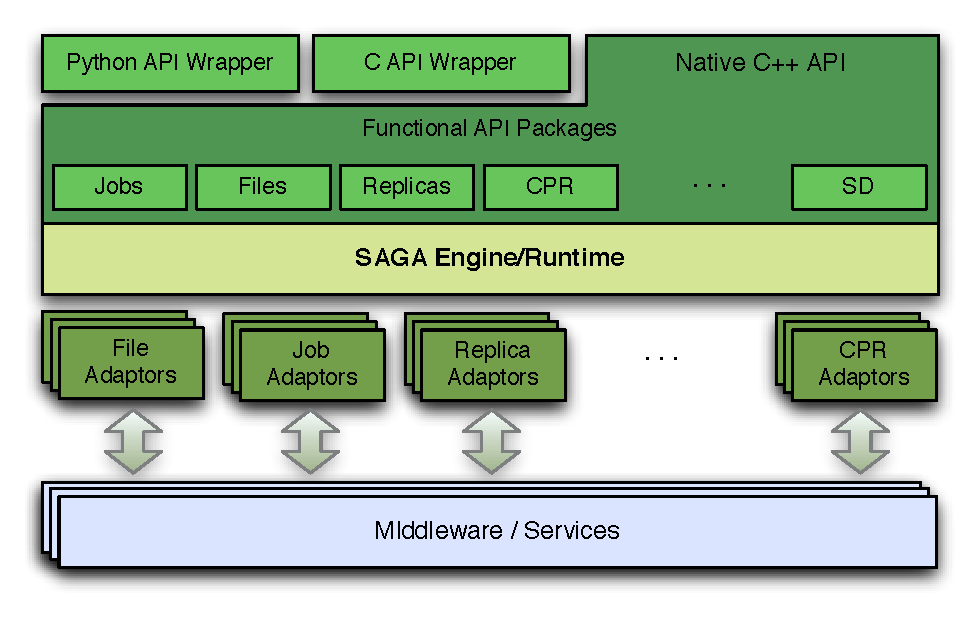
\includegraphics[scale=0.5]{stci-saga-figures-1.pdf}
\end{center}
%      \includegraphics[scale=0.4]{remdmanager.pdf}
 \caption{\small (Left) Layered schematic of the different components
    of the SAGA landscape.  Middleware specific adaptors applications
    developed using SAGA make applications developed using SAGA grid
    portable. (Right) Schematic showing the different ways in which
    SAGA can be used to develop distributed applications. (i) Using
    direct, simple SAGA calls to implement distributed functionality;
    (ii) Coordinating multiple components of an application, either
    directly, or using high-level APIs; (iii) Through the use of
    frameworks which provide either application-level usage modes,
    patterns and thus shielding the application from directly
    interfacing with the infrastructure.  SAGA facilitates the
    creation of a framework made up of ``abstractions'' (Bigjob;
    ManyJob) that supports the functionality desired for distributed
    applications, but not confined to a specific infrastructure.  The
    BigJob abstraction provides the capability to cluster sub-jobs
    into a larger big-job, and acts like a Pilot-Job. The
    abstractions, enable the allocation of resources to an application
    and not to a specific job.}
 \label{sagalayer}
\end{figure}

A fundamental question at the heart of all scientific applications, is
the question of how scientific applications can be developed so as to
use as broad a range of infrastructure as possible, without vendor or
middleware lock-in, yet with the flexibility and performance that
scientific applications demand. The SAGA programming system has been
developed to address precisely these questions, and consists of a
high-level application-oriented API, the SAGA {\it Engine} (a dynamic
library implementing the functionality of the API), and backend,
system-specific adaptors.  Our recent work using
SAGA~\cite{saga-papers} has overcome a traditional limitation of RE
simulations, viz., restricted set of platforms have been used and
consequently, only small physical systems have been investigated so
far. We have developed a general-purpose framework that can overcome
traditional limitations and can be used over a wide-range of
production distributed environments~\cite{saga-royalsoc} (and
Fig.~\ref{fig:REMD-Manager-architecture}).  Interestingly, the same
framework can be used to marshall different types and sizes of
resources~\cite{saga-papers}. For example, the BigJob abstraction that
we first employed on 512-node Linux Clusters on LONI can also be used
for monolithic usage on the 64,000 core mammoth Ranger(TACC)
machine~\cite{saga-iccs09}.  It is also important to mention that the
SAGA-based framework discussed is extensible, in that it can be used
to implement many other applications in addition to those discussed
here.

The power to do so arises from simple design decisions: the use of
appropriate programmatic and system abstractions that allow users to
do what they can do best (i.e., provide the simulation and
orchestration logic), whilst ensuring that the middleware used
provides required services (such as checkpoint management, application
monitoring and recovery) seamlessly and effectively from the
application developers perspective. 

Ensembles must be synchronized at each assimilation step. This makes
the inversion process as slow as the slowest member. This might be
addressed using (a) adaptive resource allocation and intelligent
queuing; (b) use of subensembles, possibly adaptively; (c) adapting
ensemble size.  Thus there that there is a distinct advantage of going
distributed.  It is also useful to note that for the end-user, the
complexity of using one resource is the same as using multiple
resources; however, the gains increase with every added resource.

\begin{figure}[ht]
    \centering
    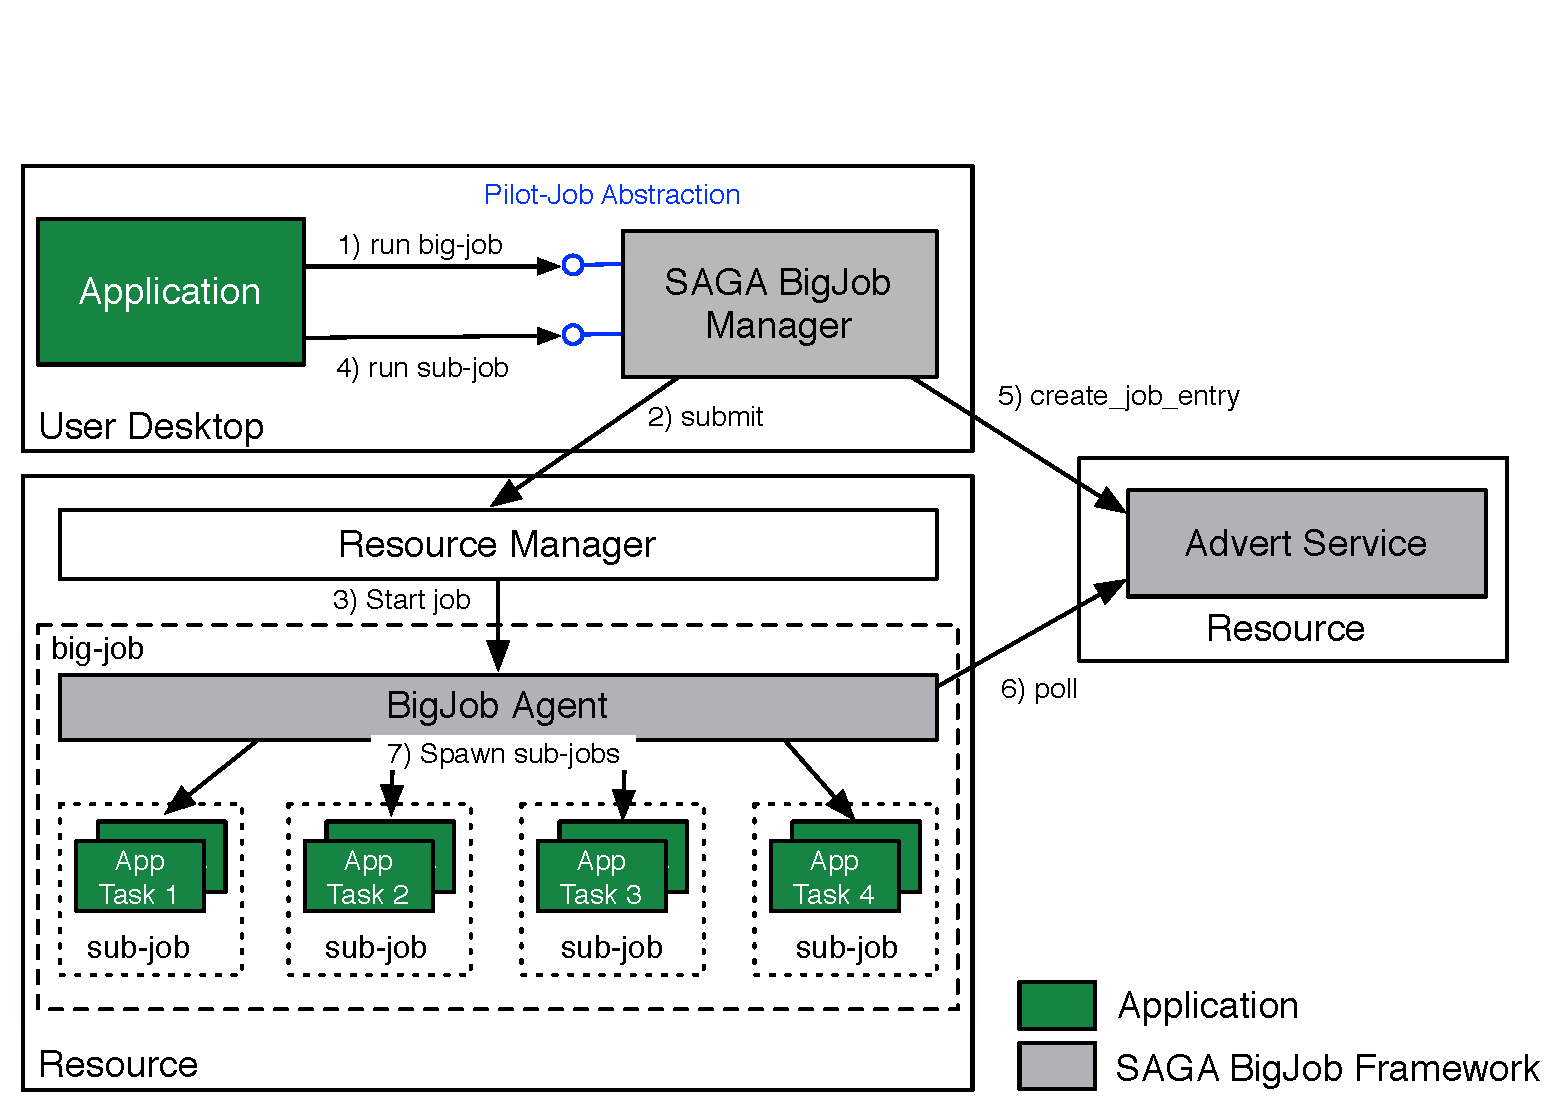
\includegraphics[width=0.66\textwidth]{./bigjob.pdf}
   \caption{BigJob Architecture: The core of the framework, the
      BigJob Manager, orchestrates a set of sub-jobs via a
      BigJob Agent using the SAGA job and file APIs.  The
      BigJob Agent is responsible for managing and monitoring sub-jobs.\up}
   \label{fig:bigjob}
\end{figure}

% \jhanote{Motivate why we need to use BigJob and Condor-GlideIn. The
%   variability of sub-job sizes and requirements. We use BigJob on TG
%   and Condor Glide-in on Condor resources}.

\begin{figure}
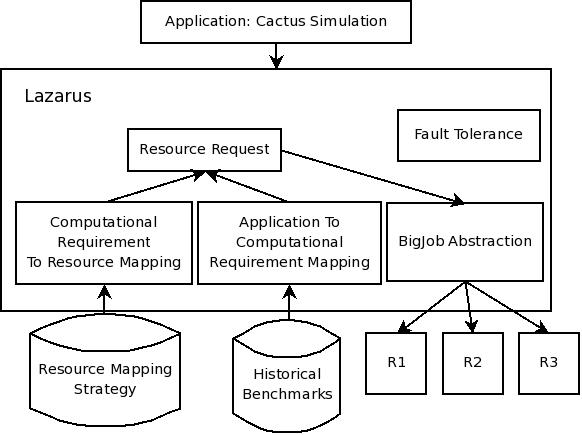
\includegraphics[scale=0.33]{Lazarus_01.jpeg}
\includegraphics[scale=0.44]{Architecture.png}
\caption{Architecture of Lazarus -- a Framework for Developing
  Autonomic Computational Science Applications. The ``Resource
  Mapping'' Strategy input is provided by BQP. Given the size of the
  individual tasks, the ``Historial Benchmarks'' help determine the
  size of the sub-jobs. (For the specific workload chosen, it so
  happens that the size of each sub-job is 16). [R] Block diagrams
  outlining how Lazarus relates to other SAGA components. Lazarus is
  built on several components: BigJob abstraction, SAGA file adaptor,
  BQP python wrappers and fault tolerance functions that are based on
  SAGA python bindings, BQP command line tools and HDF5 tools
  respectively.}
\label{fig:application_architecture}
\end{figure}

% \begin{figure}
%   \begin{center} \includegraphics[scale=0.5]{./figures/Architecture.png} 
%     \caption{Block diagrams outlining how Lazarus relates to other
%       SAGA components. Lazarus is built on several components: BigJob
%       abstraction, SAGA file adaptor, BQP python wrappers and fault
%       tolerance functions that are based on SAGA python bindings, BQP
%       command line tools and HDF5 tools
%       respectively.}\label{fig:application_architecture}
% \up\up\up\up\up\up\up%\up\up\up\up\up
% \end{center}
% \end{figure}

Lazarus utilizes SAGA, SAGA-based abstractions (BigJob) and provides
an autonomic, self-configuring, self optimizing, self monitoring and
self-healing job manager that facilitates the launch of history
matching studies on distributed high performance, high throughput and
grid computing resources ~\citep{gmac}.

Lazarus uses the BigJob abstraction to launch simulations,
the SAGA file adaptor python bindings to move files from one machine
to another and BQP data from a small python wrapper around the BQP
command line tool to retrieve the optimal location and number of
BigJobs required to satisfy the computation power required

The Lazarus framework contains several aspects of autonomy: it has
self-configuration (deployment on resources), self optimization (using
BQP data), self monitoring (checking its own output) and of course
self healing (resubmission of faulty simulations). These aspects have
been implemented with varying level of intelligence: the self
optimization for example is a basic algorithm that uses BQP data to
assign big-jobs to resources, but does not take into consideration
bandwidth requirement and the cost of copying files across
machines. The self-healing on another hand can typically resurrect
jobs that fail due to node failure as opposed to software
failure. Many autonomic features of Lazarus will be improved to
incorporate sophisticated inherent intelligence.

For runs distributed across several machines, Lazarus needs to gather
the data from all different machines into one location where the EnKF
can run. To that end, the python bindings to the SAGA file adaptors
are used to copy files over to the resource where the EnKF will run,
and copied back to all other resources after the analysis stage. Since
we are not working with a large scale production history matching run,
the amount of data transfer involved does not impose any noticeable
performance issues. Naturally, investigating the optimal location for
placing the EnKF application, based upon network performance and
real-time performance as discussed in Ref.~\cite{escience07}, will
find its way into the next iteration of Lazarus implementation.

Lazarus also uses non-SAGA components, such as a small python wrapper
for BQP. This allows Lazarus, namely its resource management function,
to query BQP for the ``optimal'' job size and duration for any given
resource. Lazarus also uses a user specified check for the integrity
of the simulation data. In our case, this is done through various
system and HDF5 calls to make sure the files exist, are not sized
zero, and a user specified command using HDF5 tools (h5ls) returns
successfully.

Lazarus is distinct to other well established and successful
approaches such as Accord~\cite{accord} for autonomic computing, in
that it is not a component-based programming system but it is a
framework already composed of multiple components. Importantly the
programming system that is used is SAGA -- both for the application
and the Lazarus framework.


\subsection{Sensors-to-Simulations (S2S)} 

To perform realtime reservoir characterization and forecast, live
sensor data must be retrieved from the field and used in the data
assimilation stage. The availability of new data also triggers a new
EnKF stage in the workflow. To that end we implemented a communication
layer based on data streaming from the data acquisition (sensor)
platforms to a data spool in the form of a MySQL database
~\ref{fig:SensorRelay}. The EnKF application queries the data spool
for the latest available sensor platform (field observations)
data. Once the new field observations are retrieved they are labeled
as ``assimilated'' to differentiate them from the next--in--line
observations.  Developed, initially using Cactus and database
interfaces, to send measurement-while-drilling (MWD) data from
drilling bottom-hole-assemblies to drill-string simulators, the S2S
framework has been extended to accommodate sending sensor data to the
BlackOil reservoir simulator (production data required for well
modelling) and the Ensemble Kalman filter for history matching. The
S2S framework also announces the arrival of new history data to
Lazarus to trigger the launching of a new stage of ensemble
simulations ~\citep{Duff1,Duff2}.  It is worth mentioning that while
currently we use a MySQL database, a more consistent solution would be
to use the SAGA advert service, which would remove the need to access
MySQL in Lazarus.

\begin{figure}
\begin{center}
 \includegraphics*[scale=0.33,angle=0]{figures/DetailedSensorFlow.png}
\end{center}
\caption{Schematic illustrating the interaction of BlackOil, EnKF, S2S
  and Lazarus. The blue arrows represent the flow of simulation data
  while the red arrows represent the flow of sensor data. % \jhanote{We
%     need a better figure than this. Where is the graffle figure that
%     you promised? Chris White is a step ahead of you in that he uses
%     graffle.. ahem}
}
\label{fig:irregular_execution}
\end{figure}

{\it Putting the Components together: } The use of an intermediate
data--spool is necessary for many reasons: it is difficult to
guarantee resource availability and synchronization with the EnKF. It
is also prohibitively costly to maintain an active EnKF session
throughout the life--time of the reservoir. With a data--spool we can
also adjust the update rate at the EnKF session without losing any
data from the reservoir. Updates to the models can be as immediate as
the moment data is broadcast from the sensors in the field, or as late
as when the reservoir is being abandoned. With immediate model
updates, we can run forecast studies.

When used in conjunction, these components allow us to perform
real--time characterization studies of large scale reservoirs
as well as long term forecast, enhanced oil
recovery and CO$_2$ sequestration studies. As more reservoir history
data is generated during enhanced oil recovery and CO$_2$ injection,
the closed-loop can continue to run and provide insight as the
reservoir geological models are being updated by the EnKF.
Continuously running the latest models in forecast simulations with
the latest sensor data will hopefully allow us to predict un-intended
movement of CO$_2$, leaks into aquifers, critical pressure build-ups
or huge pressure drops (fractures, blow-outs etc.). To that end we use
the BlackOil reservoir simulator as an early prototype of what will
eventually be an accurate simulator that can model CO$_2$
sequestration, geochemical and geomechanical phenomena. The S2S
framework is also under heavy development to add sensor metadata
allowing Lazarus, through autonomic logic, to distinguish between
critical and non-critical sensor data, and ultimately making use of
on-demand computing resources (should the sensor data prove critical).


\section{Performance Data and Analysis:} 

We have previously run an EnKF based application on several TeraGrid
resources and demonstrated effective {\it Scale-out} across three
machines~\citep{gmac}.  Additionally, we incorporate the use of Condor
pools in Lazarus for even higher throughput, demonstrating possible
advantages to using multiple pilot job mechanisms. % \jhanote{mention
%   that although this is for HM, the performance numbers are valid for
%   Sequestration problem too.}

\subsection{Performance Data} 

\begin{figure}
\begin{center}
  \includegraphics*[scale=0.5,angle=0]{figures/Figure7.png}
\end{center}
\caption{Time to completion with Lazarus. From Left to Right: (i)
  Ranger (ii) Ranger when using BQP, (iii) QueenBee, (iii) Ranger and
  QueenBee, (iv) Ranger, QueenBee and Abe, (v) Ranger, QueenBee and
  Abe when using BQP.}
\label{fig:SingleVsDistributed}
\end{figure}


% \jhanote{We could either reproduce the above data plot as is, or we
%   could extend the data plot to include $T_c$ when Purdue's Condor
%   Pool is introduced into the mix. I think there is some merit in
%   extending to scale-out onto 4 resources (R, Q, A + Purdue) --
%   obviously without worrying about BQP. We don't have to use BigJob on
%   the Purdue-Condor pool}\yyenote{No time...}

In this work, in addition to a different scientific problem, we
integrate (simulated) sensor data into the computational loop; the
time-dependent sensor-data dynamically drives the application, and
influences the controls and execution trajectory in phase-space.

These are amongst the first simulations
that use general purpose frameworks (as distinguished from specialized
frameworks, for example LEAD) on production infrastructure.

\subsection{Resorvoir Characterisation}

After several iterations of the workflow and the convergence of the
EnKF to within a fixed value, a 3D map of the permeability (a measure of the flow
of the rocks) and porosity (a measure of the capacity of the rocks) is 
output and defines the properties of the reservoir to a first
approximation. \begin{figure}
\begin{center}
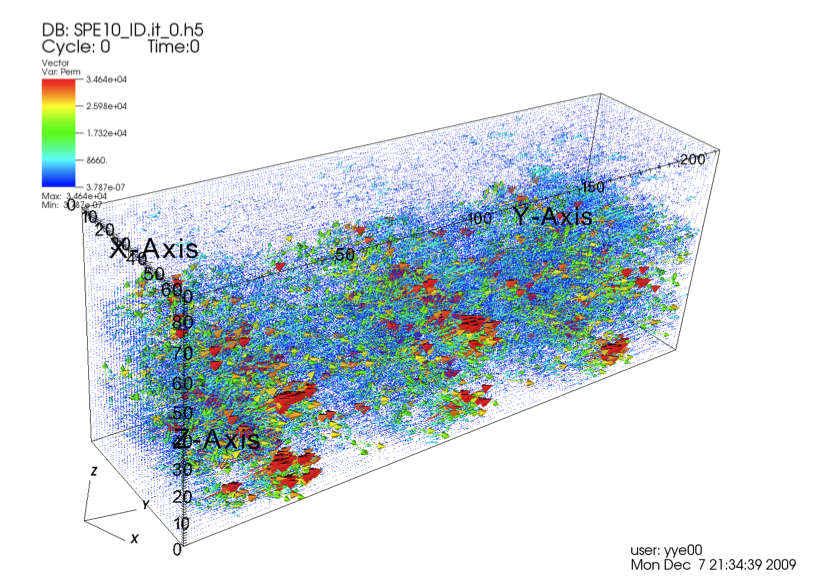
\includegraphics[scale=0.45]{figures/permeability.png}
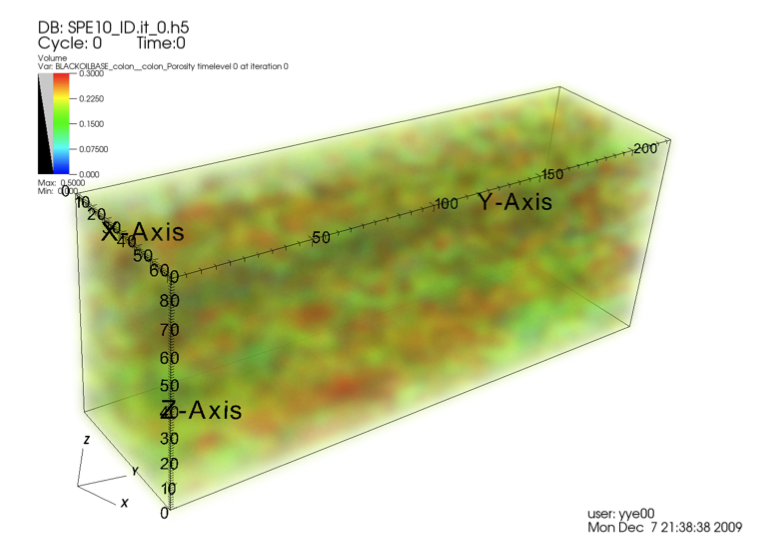
\includegraphics[scale=0.45]{figures/porosity.png}
\end{center}
\caption[Simulation Output]{[L] Resorvoir as characterised by the
  permeabilty, and [R] porosity. }
\label{}
\end{figure}

\subsection{Analysis} 

The next step is to determine what is the extent of sequestration in a
reservoir characterised by the porosity and permeabilty.  The answer
to this is provided by the relative proportion of CO$_2$ per grid
cell. Figure 7 provides a measure of this relative proportion for the 
reservoir characterised in Figure 6. Fig 8 provides a quantitative
estimate for how the injection varies with time for 10 rather similar
models. 

\begin{figure}
\begin{center}
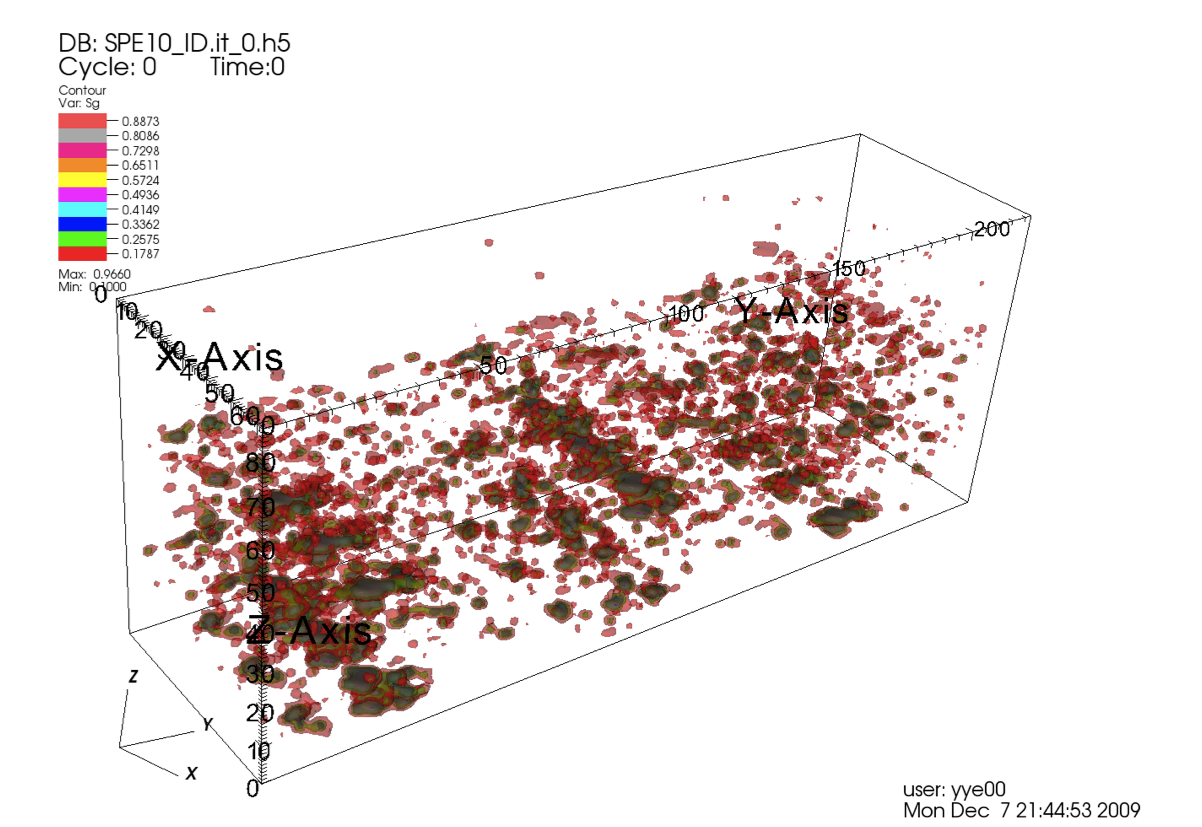
\includegraphics[scale=0.6]{figures/saturation.png} 
\end{center}
\caption[Simulation Output]{The saturation (relative proportion) of
  CO$_2$ for the reservoir characterised in Fig 6.}
\label{}
\end{figure}

\begin{figure}
\begin{center}\
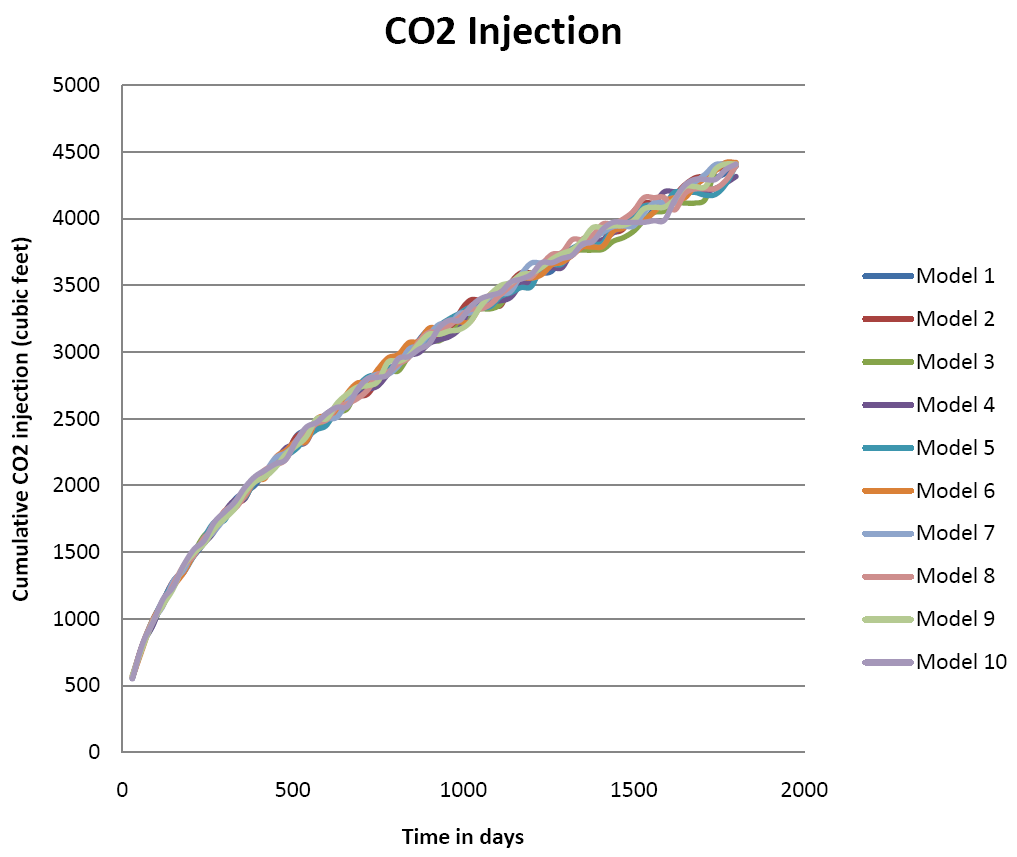
\includegraphics[scale=0.33]{figures/co2seq.png}
\end{center}
\caption[Simulation Output]{Simulation output of the injection of
  CO$_2$ as a function of time since start of injection. The output for 10  different models are
  plotted, showing the sensitivity of the injection amount to the
  underlying model. \jhanote{need to define time in days.. for what?}}
\label{fig:SensorRelay}
\end{figure}

% \jhanote{In this section we revisit the ``computational requirements
%   of real problems'' as set out near the beginning. We then calibrate
%   requirements based upon our results here -- showing (i) that we have
%   met a fraction of the requirements, but, (ii) that we need to do
%   much more in order to be able to meet the requirements laid out for
%   real problems.}

{\it Conclusion: }A triad of unique aspects are developed in this
paper: (i) We incorporate the use of EnKF in reservoir
characterization for carbon dioxide sequestration studies, combining
two developing research areas and investigating the forefront (ii) We
extend our EnKF based approach further with the incorporation of live
sensor data that influences the entire study (iii) We establish the
ability to {\it scale-out} to a large number of distinct heterogeneous
resources.

The focus of this paper has been on developing the high-performance
and distributed cyber-infrastructure required to simulate the CO$_2$
sequestration properties of a reservoir. The aim has not been to
perform a detailed analysis or analyse the underlying scientific
problem, but to derive the infrastructure requirements from the
scientific requirements, to implement a solution and to validate our
solution. This is consistent with an application-oriented
cyberinfrastructure development philosophy.


\bibliographystyle{kluwer}
\bibliography{cseq_abstract}
\end{document}


\item \yyenote{ The problem is performing reservoir studies that are
    updated real-time, the application is the history-matching,
    forecasting and CO2 sequestration scenario. We want to use
    cyberinfrastructure because of several reasons: we have many
    simulations of complex reservoirs, that means we have to go
    parallel for higher throughput and use parallel processing. To be
    able to do this in real-time i.e. as the sensor data streams in,
    we have to have very fast turn-around for simulations that means
    high throughput, so we use everything at our disposal including
    grids which so far works. Other motivation, and this is more of a
    petroleum engineering perspective: if we cannot make use of
    existing tools and technologies today, chances are we will not be
    able to use new tools and technologies of tomorrow. We can
    elaborate on how we need cyberinfrastructure not just cycles: HPC
    for the simulator, grid and high throughput for many simulations
    and bigjob, databases for the sensor data i.e. data driven and
    data aware for Lazarus, as well as restart/fault-tolerance
    mechanisms, and of course sensors in the field. Now all I have to
    do is structure this so that it resembles a half defence
    paragraph. }

 \item Sensor driven application and workflow: the number of stages is controlled by 
sensors and the simulations themselves use sensor data

 \item Highly unpredictable: we have workflows that are changing dynamically and 
applications that use parameters from live data that we do not see before, everything will 
vary wildly


\item The sensor data can be quite critical: if you are injecting CO2
  and suddenly (i.e. real-time suddenly) you lose well-head pressure:
  the CO2 is going somewhere, you want to find out where! It could be
  building up around the casing or going into a fracture, really nasty
  stuff can happen \jhanote{elaborate addressed} \yyenote{The sensor
    data can contain critical information: pressure went to the roof
    or pressure went to zero, i.e. bad things will happen. We need to
    be able to identify these situations because for those cases
    obtaining simulation results ASAP is very important}

\item Sensor data can be simply faulty: a blown out fuse, a bad relay,
  and you get let's say pressure of -5 billion psi, quite
  nonphysical. Instead of wasting SU's on these bad things we need to
  halt and report the issue. Hence we need some form of intelligence
  to the sensor data: either through XML description of
  allowable/permissible ranges of the data, what range is normal, what
  range is critical and what range is abnormal (or faulty) and so
  on. Instrumentation engineering is a big discipline and what we are
  trying to do here is apply autonomic instrumentation awareness: the
  simulation and EnKF do not just pull data, they pull information,
  and some autonomy in reasoning what the information is is highly
  desirable (but lacking right now). This probably needs to be moved
  later on and put in the future work for the actual paper for
  e-science and maybe if I get time to work on this for the eventual
  paper for UK-escience.

\item While the application in this case is CO2 seq, this can be really anything in the real world EnKF for atmospherics, EnKF for radar, or simply hurricane simulations 

\item Keeping tabs, book-keeping is incredibly difficult, you will need to archive data effectively for larger runs (list this in the challenges) \item In terms of autonomics, we have: sensor driven workflow (i.e. throughput), sensor driven simulations, i.e. data-aware workflows and data-aware simulations. We do not have this now but a natural extension is checking whether the data is critical or not, this would make the application data-criticality aware (not just availability of data but nature of the data... need better term for that one) \jhanote{this needs a bit of clarification} \yyenote{a pressure loss of let's say -5 psi is not the same as -5000 psi, one would not cause panic the other would. It is a good idea to have a person at the helm who would notice that big of a drop and realize: hey we need the results of those simulations immediately, and jump the queues or do something special. What would be even great: Lazarus is made aware of this, does things so that everything is optimized for faster turnover and results are on hand asap. If the clarification is the application of EnKF: the method has its origins in atmospherics: radar, hurricane tracking, meteorology that sort of thing. This not being my domain I do not know much about it but all books on EnKF say this}

\item Need for autonomics is driven by the requirement to either respond to external sensors or internal compute data-output. \jhanote{Elaborate on how this arises, what this means..}

\item Input data drives the priority of the next state of simulations, based upon state of the application

\item We have (or will have soon once the admins fix it) condor, that should help with the on-demand computing issue by allowing us to harvest cycles for regular jobs and put the critical ones in the high-priority queues

\item One interesting feature: when we run this we are doing 2 things: history match then forecast, i.e. we are updating our ``study'' of the reservoir behavior dynamically as it evolves in realtime

\item Need to formulate the problem in terms of Application Objective, Mechanisms and Strategy.

\item Need for distributed computing when urgent -- ``little bit on
  all machines''. Need for autonomic decision making in determining
  the resource: Lazarus determines where to send the
  simulation. \jhanote{We need to say something about how this
    decision could be made in practise} \yyenote{Was hoping Ole's
    scheduling stuff would help, I have no idea how to begin to
    optimize this, perhaps a reverse scheduler? I don't know honestly}
  \jhanote{OK let us leave this out}

\item Application objective: match-making for ; mechanism:  Lazarus.. etc ; strategy: 

\end{itemize}

\section{Introduction}

The sensor data can be quite critical: if you are injecting CO2 and suddenly (i.e. real-time suddenly) you lose well-head pressure: the CO2 is going somewhere, you want to find out where! It could be building up around the casing or going into a fracture, really nasty stuff can happen
\begin{itemize}
 \item Based on that, we will need several things: frequent and dynamic updates of available sensor data (i.e. sensor platform, which we sort of have but needs more work, this is LabVIEW side...)
 \item On demand computing: You want to know if the CO2 is just moving to new places normally (i.e. you have low permeability and have to cross a threshold to get CO2 through there) or you broke the rock and CO2 is building around the casing of the well and the whole damn thing will explode
 \item Special handling of critical sensor data: we might need some
   sort of mechanism to distinguish low priority sensor data from
   critical sensor data, based on that, throw a token for spruce or
   switch to dedicated queues or something like that
 \item The data is sensitive and confidential, security is a big issue that we will need to address, same goes for database redundancy (you don't want all ensembles hitting a single DB for latest sensor data all at once, you want redundancy...)
\item Based on sensor data, we might want to run fire control models, emergency response models, kill-well/well-shutdown models etc... So analysis of sensor data before we jam it in the workflow might be important
\end{itemize}
}

% \begin{figure}
% \begin{center}
% 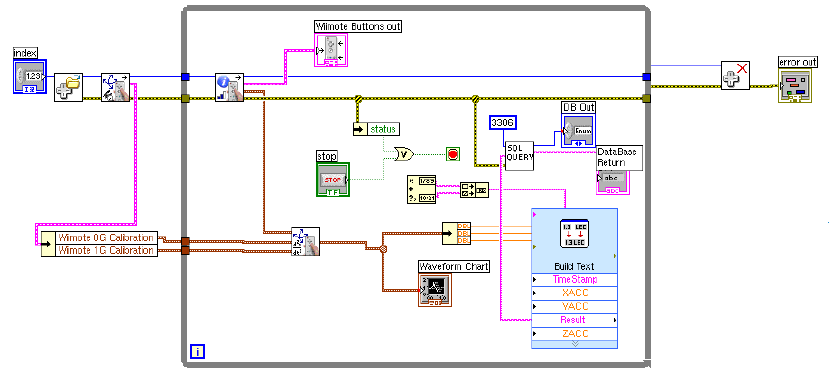
\includegraphics[scale=0.65]{./figures/LabView.png}
% \end{center}
% \caption[Sensor side LabVIEW vi]{Sensor side LabVIEW vi. To stream data from sensor platforms to data spools we use a LabVIEW vi that makes calls to a shared library containing an interface to the database (MySQL). Initial tests were conducted using a Wii mote 3--axis accelerometer. Image courtesy of Richard G. Duff }
% \label{fig:LabView}
% \up
% \up
% \end{figure}

% Special care had to be taken when interfacing to sensor platforms:
% there is no unified specification for communicating abstract sensor
% information. The simplest approach was to develop an interface to a
% common data acquisition application: LabVIEW from National
% Instruments ~\cite{LabVIEW}. To that end we developed a virtual
% instrument (vi) that makes function calls to a shared library which
% in turn interfaces to the MySQL database (Figure
% ~\ref{fig:LabView}). The vi has an adjustable streaming rate for
% polling sensor information and relaying it to the database, and is
% modular so it can be integrated in existing vi's as a sub--vi. This
% translates to painless integration with existing field and
% laboratory sensor platforms, in particular, the UCoMs sand tank
% experiment ~\cite{UCOMS}.

%It is worth mentioning that the intention here was to develop an
% abstract interface to sensor data that can accommodate everything
% from drill--string modelling ~\cite{DrillingLab}, well--heads,
% weather stations and buoys. This is one of the reasons why a ProdML
% ~\cite{ProdML} was not the first choice of interfaces. However,
% should the need arise, we can develop a direct ProdML to PETSc
% interface which will have no significant impact on the closed loop
% performance.




